\section{Verteilung der Anwendung}
\label{subsec:implementation:ApplicationDistribution}
Ein wesentliche Anforderung an die Praxisanwendung ist dem Anforderungskatalog unter Kapitel \ref{sec:Eruierung:technicalRequierements} entsprechend, die Fokusierung der Architektur der Software auf Verteilung. Um dies zu erreichen wurde bereits die Anwendung in verschiedene Services unterteilt. Diese wurden in Abschnitt \ref{sec:implementation:serviceAndComponentOrientation} näher beschrieben. \\
Für die Instanziierung einer Komponente wurden vier verschiedene Konsolenanwendungen implementiert. Wobei für jeden Service ein eigene Anwendung geschrieben wurde, mit Ausnahme vom \textit{Domain-Service} und \textit{Command-Service}, welche in einer gemeinsamen Anwendung operieren. \\
Die Verbindung zwischen den einzelnen Komponenten wird mit der Cluster Unterstützung, welche \textit{Akka.net} bietet und in Abschnitt \ref{subsec:implementation:akka:cluster} beschrieben ist, umgesetzt. 

\subsection{Cluster}
\label{subsec:implementation:akka:cluster}
Die Cluster Funktionalität von \textit{Akka.net} bietet die möglichkeit zusammengehörende Anwendungen über ein Netzwerk zu verbinden und somit ein Cluster zu formen. Für den Benutzer der Anwendung harmoniert der Cluster als eine Einheit. Dazu wird mittels einem \textit{Peer-to-Peer} Netzwerk jede Teilnehmende Anwendung mit jeder anderen verbunden. Über ein Protokoll, das sogenannte \textit{Gossip} Protokoll, genauer beschrieben in Abschnitt \ref{subsec:implementation:gossip}, werden Informationen zum Zustand des Clusters ausgetauscht. Jede am Cluster Teilnehmende Anwendung wird als Node bezeichnet. Somit bilden zwei oder mehr Nodes einen Cluster. \\
Jede Anwendung bekommt Rollen zugewissen, welche es zur Laufzeit übernehmen kann. Eine Rolle definiert in \textit{Akka.net} ein Aufgabengebiet innerhalb des Clusters. Für \textit{TyrolSky} wurden die fünf bereits definierten Services in Abschnitt \ref{sec:implementation:serviceAndComponentOrientation} als Rollen herangenommen. Tritt eine Anwendung dem Cluster bei, so gibt sie zu Beginn bekannt, welche Rollen sie im Cluster übernehmen kann. Eine Rolle kann somit mehrfach im Cluster vorhanden sein. \\
Die Kommunikation zwischen den Komponenten erfolgt innerhalb des \textit{Akka.net} Cluster entweder über Routing Mechanismen, siehe Abschnitt \ref{subsec:implementation:akkaRouting} oder über verteilte Daten, welche in Shards organisiert sind, siehe dazu Abschnitt \ref{subsec:implementation:akkaSharding}. 

\subsection{Routing}
\label{subsec:implementation:akkaRouting}
In Kapitel \ref{sec:actor:patterns:routing} wurde bereits darauf eingegangen das es in einem System Actors geben kann, welche für die Verteilung von Nachrichten zuständig sind. Die Verteilung von Nachrichten in einem auf \textit{Akka.net} Cluster aufbauenden System wird durch eben solche Router bewerkstelligt. \\
Das Framework bietet dabei bereits verschiedene Typen von Actors an, welche Nachrichten annehmen und an andere Actors auf entfernten Nodes weiterleitet. Diese, auf das weiterleiten von Nachrichten spezialisieren Actoren, werden Router genannt. Bei der erstellung eines Routers wird über Parameter angegeben, welche Actoren als Ziel dienen können und welche Routingsstrategie verwendet werden soll. Weiters können die möglichen Rollen, auf welchem sich die Ziele befinden, eingeschränkt werden. Nachfolgend wird die verwendeten Routingsstrategie innerhalb von \textit{TyrolSky} beschrieben. \\
Sämtliche Anfragen an das System haben ihren Startpunkt bei der Komponente \textit{API-Service}. Von dieser müssen Anfragen an die betreffenden Komponenten weitergeleitet werden. Diese können, da die Anwendung mit dem \textit{CQRS} Prinzip arbeitet sich nur in den Rollen \textit{Command-Service} und \textit{Query-Service} befinden. Bei einer ankommenden Anfrage kann der \textit{API-Service} aufgrund der Anfrage entscheiden ob die weitere verarbeitung in einem \textit{Query} oder \textit{Command-Service} stattfinden soll. Dementsprechend wird die Anfrage an den Router, welcher für den entsprechenden Service zuständig ist, weitergeleitet. Der Router überwacht nun mithilfe der Informationen welche er über \textit{Gossip} erhält, den Status von anderen Nodes im Cluster. Empfängt der Router eine Nachricht, so kann er einen der in Frage kommenden, verfügbaren Nodes auswählen, und die Nachricht diesem zustellen. \\
Bei der Auswahl des Nodes wird dabei für diesen Router das \textit{Round-Robin} Verfahren eingesetzt. Somit ist eine gleichmäßige verteilung der Nachrichten auf die unterschiedliche Host möglich. Es gibt neben dem \textit{Round-Robin} Routing Verfahren noch andere bereits implementierte Routingsstrategien innerhalb von \text{Akka.net} wie unter anderem Zufälliges Routing, Hashingrouting und andere. Jedoch wurden diese im zuge der Umsetzung von \textit{TyrolSky} nicht verwendet. \\
In Abbildung \ref{fig:implementation:routing} ist das zusammenspiel der drei Komponenten \textit{API-Service}, \textit{Query-Service} und \textit{Command-Service} zu sehen, wobei von den zwei letzt genanten jeweils zwei Instanzen am Cluster teilnehmen. Die Router auf dem Node \textit{A} leiten die Nachrichten abwechselnd an die zwei Nodes \textit{B} und \textit{C} oder an \textit{D} und \textit{E}. 

\begin{figure}
    \centering
    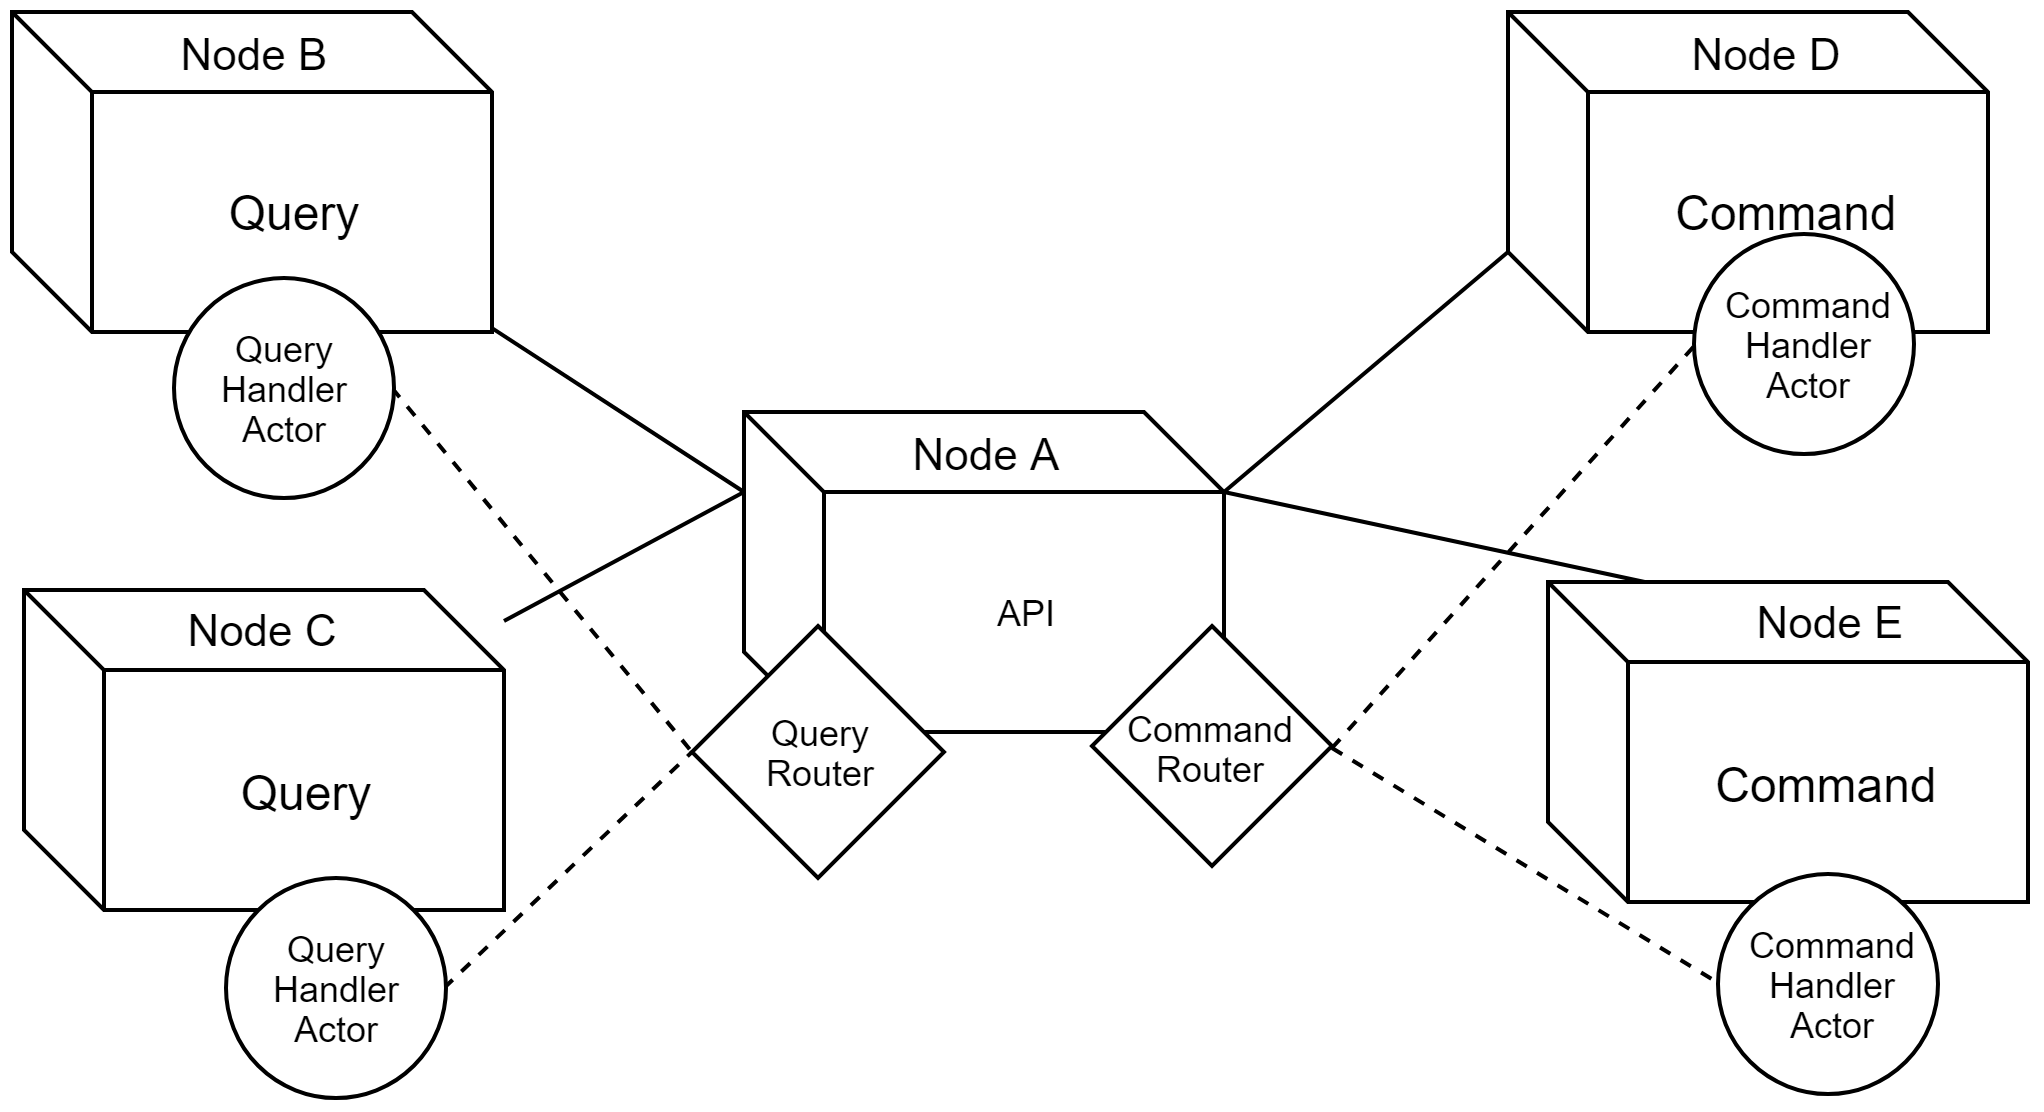
\includegraphics[width=\linewidth]{gfx/implementation/ClusterRouter}
    \caption{Ein verteiler \textit{Round-Robin} Router welcher Nachrichten von der Komponente \textit{API} auf andere Komponenten verteilt.}
    \label{fig:implementation:routing}
\end{figure} 

\subsection{Gossip}
\label{subsec:implementation:gossip}
Bereits in Abschnitt \ref{subsec:implementation:lighthouse} wurde die Komponente \textit{Lighthouse} vorgestellt, welche als Einstiegspunkt für alle Nodes verwendet wird. Die Verbindung zu den restlichen im Cluster vorhandenen Nodes, wird über das \textit{Gossip} Protokoll hergestellt. \\
Der Name \textit{Gossip} leitet sich vom Geschwätz mehrerer Personen ab, jeder erzählt einem anderen etwas, und so wissen alle über jeden anderen  bescheid. Das gleiche Prinzip wird in diesem Protokoll verwendet, um Änderungen an einem einzelnen Node allen anderen Nodes im Cluster bekannt zu geben. \\
Nodes mit der Rolle \textit{Lighthouse} sind der Start dieser Kommunikation. Deshalb müssen diese Nodes auch über eine fixe Adresse verfügen, im Fall von \textit{TyrolSky} sind das Ip-Addresse und Port. Komponenten welche nun dem Cluster beitreten wollen, melden sich bei einem der \textit{Lighthouse} Komponenten an, und geben bekannt über welche Adresse sie erreichbar sind. Über das \textit{Gossip} Protokoll wird nun jedem bereits im System beigetretenen Node mitgeteilt das sich ein neuer Node im Cluster befindet. \\
In der Kommunikation zwischen den Nodes wird den anderen Nodes auch mitgeteilt, welche Rollen eine Komponenten besitzt. Dies wird dann anschließend von den Routern, siehe Abschnitt \ref{fig:implementation:routing}, verwendet, um Nachrichten an die diese Rollen zuzustellen. Weiters beinhaltet das Protokoll auch Informationen über den Zustand der einzelnen Nodes. Bei einer fehlerhaften Verbindung zwischen zwei Nodes werden alle anderen Nodes über den Fehlerzustand benachrichtigt. Ist ein Node nicht mehr erreichbar ohne das eine kontrollierte abmeldung vom Cluster stattgefunden hat, kann er jedoch nicht einfach aus dem Cluster entfernt werden sondern es muss eine Lösungsstrategie implementiert sein, siehe dazu den nachfolgenden Abschnitt \ref{subsec:implementation:splitBrain}. \\ 
Das Protokoll dient neben der Zusammenfügung der einzelnen Node zu einem Cluster auch zum austausch von Informationen über den aktuellen Zustand des Clusters. Muss vom Protokoll eine entscheidung getroffen werde, wie beispielsweiße die Entscheidung über den Beitritt zum Cluster, wird ein Node ausgewählt, welcher die Führung über den Cluster übernimmt. Im Fall von \textit{TyrolSky} ist das immer der ältester Node im Cluster, wird dieser vom Cluster entfernt, übernimmt die Führung der nächst älteste Node.  

\subsection{Split Brain} 
\label{subsec:implementation:splitBrain}
Wie bereits in Kapitel \ref{sec:distributedSystems:capTheorem} besprochen, kann bei eine Verbindung zwischen zwei Geräten, jederzeit ein Problem auftreten, welche die Kommunikation zwischen den Teilnehmern stört oder gänzlich unterbricht. Durch eine solche Störung ist es dem betroffenen Node nicht mehr möglich am \textit{Gossip} teilzunehmen und seinen Zustand mitzuteilen. Ebenfalls wissen die anderen Cluster Teilnehmer den Grund für trennung der Kommunikation nicht, und können dementsprechend auch keine Aussage treffen ob die trennung nur temporär ist, oder ob der gestörte Partner gar nicht mehr existiert. \\
Ein ähnliches Szenario kann auch auftreten, wenn zwei oder mehr Gruppen von Nodes zwar untereinander eine aufrechte Kommunikation führen können, jedoch die Gruppen selbst getrennt wurden. So agiert jede Gruppe des Clusters für sich selber und kann sich  mit den anderen Gruppen nicht mehr verständigen. Würde nun jeder Node im Cluster andereren Nodes welche für ihn nicht erreichbar sind, selbstständig entfernen, so würde jede Gruppe einen eigenen, neuen Cluster bilden, was als \textit{Split Brain} bezeichnet wird. Bildet sich aus einem Cluster durch gegenseitiges Entfernen mehrere neue Clusters, so bilden sich zwei oder mehrere Parallelstrukturen welche die Konsistenz der gesamten Applikation verletzen können. Unter anderem werden die Prinzipien von \textit{Cluster Singletons} oder \textit{Sharding} verletzt und dies kann wiederum zu redundanzen führen. \\
In \textit{Akka.net} gibt es bereits einige Strategieren welche für das \textit{Split Brain} Problem angewandt wurden. Jede Strategie hat jedoch einen Nachteil welcher teilweise sogar zum Stillstand der gesamten Anwendung führen kann. 

\begin{itemize}
    \litem{Statische Mehrheit}
    Jedem teilnehmenden Node wird die gleiche statische Nummer beim Start übergeben. Kann ein Node weniger Teilnehmer erreichen als die Nummer angibt, so wird beendet sich der Node selbstständig. Teilt sich jedoch das Netzwerk in mehr als zwei Gruppen auf, so werden alle Nodes im gesamten Netzwerk beendet. 
    \litem{Behalte Mehrheit}
    Wird der Cluster geteilt, wird anhand des zuletzt verfügbaren Informationen über den gesamten Cluster analysiert, ob der nun erreichbare Teil des Clusters die Mehrheit der vor der Unterbrechung  beteiligten Nodes  erreichen kann. Entspricht der neue Cluster der Mehrheit so werden die Nodes nicht beendet. Ansonsten werden alle Nodes des gesplitteten Clusters beendet. Auch hier kann das Aufteilen des Clusters in mehr als zwei Gruppen zum Stillstand des gesamten Clusters führen.

    \litem{Behalte Älteste}
    Durch das \textit{Gossip Protokoll}, siehe Abschnitt \ref{subsec:implementation:gossip}, wird  mitgeteilt zu welchem Zeitpunkt ein Node dem Cluster beigetretten ist. Darauf basierend kann berechnet werden welcher Node der älteste im Cluster ist. Sobald sich der Cluster aufteilt, werden alle Nodes beendet, welche den ältesten Node nicht erreichen können. Dadurch ist sichergestellt, das auch bei einer mehrfachen aufteilung nicht der ganze Cluster beendet wird. Wird jedoch der teil vom Node getrennt welcher den ältesten Nodes und einige wenige andere Cluster beinhalteten, so wird der gesamte größere Teil des Clusters beendet. Die Anwendung ist zwar nicht beendet, jedoch wurden mehr Nodes beendet als Nötig. 

    \litem{Behalte Referenz}   
    Es wird ein fixer Nodes bestimmt welcher erreichbar sein muss. Erreichen andere Nodes diesen nicht mehr, so werden sie automatisch beendet. Dies führt dazu, dass wenn der Referenzierte Node im gesamten Cluster nicht mehr erreichbar ist, die gesamte Anwendung beendet wird. Jedoch ist eine aufteilung in zwei Teilen unter keinen Umständen möglich.
\end{itemize}
Für die Implementierung der \textit{TyrolSky} Anwendung wurde die Strategie \textit{Behalte Älteste} gewählt. Eine zersplitterung des Clusters ist somit äußerst unwahrscheinlich. Das Risiko zu viele Nodes im Fehlerzustand zu beenden und das System somit kurzfristig zu verlangsamen wird eingegangen um die Datenkonsistenz für das Sharding nicht zu verletzen.  

\subsection{Globale Dienste}
\label{subsec:implementation:singeltons}
Bereits in Abschnitt \ref{subsubsub:implementation:queryActorModel:resultPreparator} wurde ein Actor benötigt, welcher um korrekt zu funktionieren, nur exakt einmal im gesamten Cluster instanziiert werden sein darf. Im konkreten beispiel war dies erforderlich, da der Actor für andere Actoren eindeutige, wiederverwendbare Namen generieren muss. In \textit{Akka.net} werden solche Actoren als \textit{Singletons} bezeichnet. Das Framework gewährleistet, dass die Actors welche als Singletons deklariert sind, nur einmal im Cluster vorhanden sind. Dabei wird auch berücksichtigt, dass wenn der Node, auf welchem der Singleton Actor läuft, vom Cluster entfernt wird, das Singleton auf einem anderen Node im Cluster verschoben wird. Dadurch ist der Actor, mit Ausnahme der Zeit welche der verschiebe Prozess benötigt, jederzeit im System exakt einmal verfügbar. \\
Für die Überwachung und das Management der einzelnen Singleton Actors ist der führende Cluster Node zuständig, siehe dazu Abschnitt \ref{subsec:implementation:gossip}. Jedem Singleton kann auch eine Cluster Rolle zugewissen werden, anschließend werden diese Singletons nur auf Nodes, welche dieser Rolle zugeordnet sind, ausgerollt. \\
Für die Implementierung von \textit{TyrolSky} wurden zwei Singletons eingesetzt. Beide werde für die Umsetzung die Namenverwaltung für die beiden Ergebnissaufbereiter im \textit{Query Service} benötigt.  Die zwei Singletons wurde die Rolle \textit{Query} zugewiesen,  womit sie auch nur auf den Nodes laufen, auf welchem sich die Ergebnissaufbereiter befinden.

\subsection{Verteilung transaktionaler Daten}
\label{subsec:implementation:akkaSharding}
Ein wesentlicher Teil der Komponente \textit{Domain Service}, Abschnitt \ref{subsec:implementation:domainService}, ist das Verteilen der Entitäten auf verschiedene Nodes der Rolle \textit{Domain Service}. Wie im Abschnitt über \textit{Domain Service} bereits erwähnt, wird die Verteilung der Entitäten über den gesamten Cluster mit dem Prinzip des \textit{Shardings} gelöst. \\
Die Idee hinter \textit{Sharding} basiert auf Vorgehensweisen für verteilte Datenbanken und bedeutet laut \cite{shardingCattell}, dass Daten mithilfe eines Schlüssels auf unterschiedliche Hosts verteilt werden. Dabei bekommt jeder beteiligte Host einen bestimmten Bereich der Schlüsselmenge zugeteilt. Alle Hosts besitzen die Informationen welche Schlüsselbereiche zu welchem Host zugeordnet sind und können davon ausgehen, dass der dazugehörigen Datensatz sich an dem entsprechend Host befindet. Dadurch ist eine effektive Verteilung von Daten auf unterschiedliche Hosts möglich, ohne das dabei jeder beteiligte sämtliche Daten besitzen muss. Jedoch muss für eine Abfrage immer der dazugehörige Schlüssel bekannt sein. \\
Die Implementierung von \textit{TyrolSky} benützt diese Technik mithilfe von \textit{Akka.net} um Actoren über mehrere Nodes zu verteilen und dabei sicherstellen, dass diese von jedem anderen Node erreicht werden können. Dazu werden die Entitäten, also die Actoren welche im Sharding Cluster leben sollen, in \textit{Shards} unterteilt. Auf jedem Node welcher \textit{Shards} übernehmen soll, wird ein oder mehrere  \textit{Shard Regions} gestartet. Dieser übernimmt, wie in Abbildung \ref{fig:implementation:actorSharding} dargestellt, die im zugewiesenen \textit{Shards} und startet die darin befindlichen Entitäten. Die Anzahl an möglichen \text{Shards} wird darbei für eine Anwendung fixiert. Im Falle von \textit{TyrolSky} werden {100} \textit{Shards} verwendet. Diese werden gleichmäßig an die verfügbaren \textit{Shard Regions} verteilt. Wird eine neue Region hinzugefügt, erfolgt eine Umverteilung der \textit{Shards}, womit auch die darin befindlichen Actors umverteilt werden. 

\begin{figure}
    \centering
    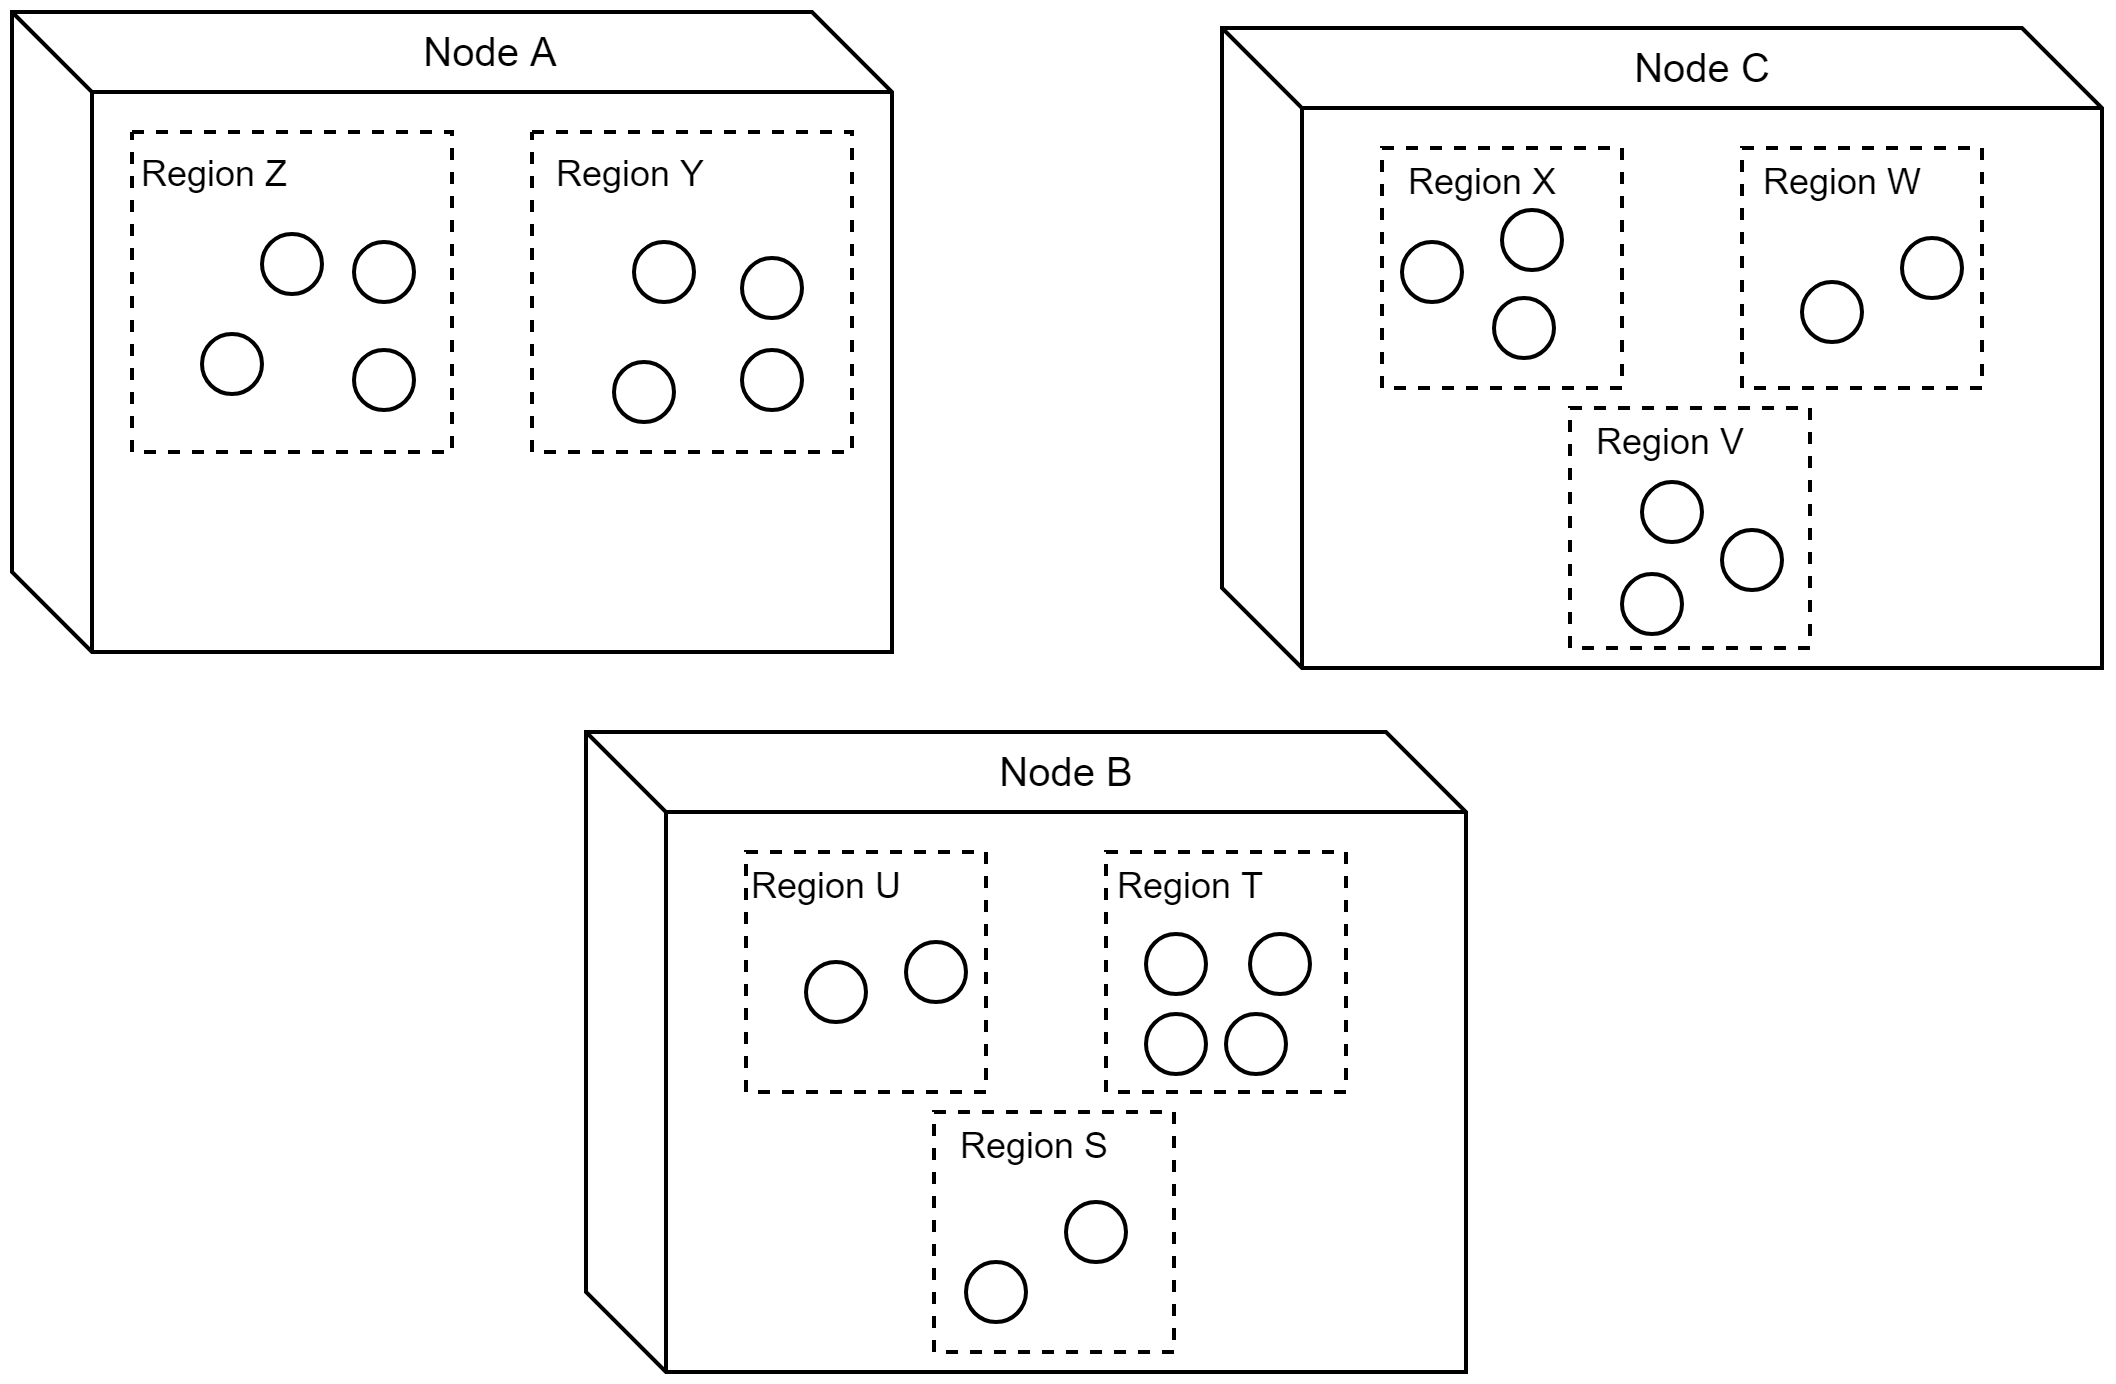
\includegraphics[width=0.8\linewidth]{gfx/implementation/Sharding}
    \caption{Verteilung von Entitäten in Shards, welche selber wieder in \textit{Shard Groups} organisiert sind. Die Gruppen können zwischen den Nodes verteilt werden. }
    \label{fig:implementation:actorSharding}
\end{figure} 

\subsubsection{Nachrichten in \textit{Shards}}
Ein Grundprinzip von \textit{Sharding} ist die Unterteilung von Entitäten in unterschiedliche Gruppen, sogenannte \textit{Shards}. Dies wird in der \textit{Akka.net} Cluster Implementierung, über die Zustellung der Nachrichten gelöst. Dazu werden Nachrichten nicht wie bei Actor Systemen direkt an den Actor gesendet, sondern zuerst an einen Sharding Manager. Diese Nachrichten enthalten eine Identifikationsnummer der Entität, an welche sie gerichtet ist. Der Manager interpretiert diese Nachricht und errechnet sich aus der Identifikationsnummer eine \textit{Shard} Identifikation. Anschließend prüft er in welcher \textit{Shard Group} sich der \textit{Shard} befindet und auf welchem Node sich diese Gruppe aktuell befindet. Anschließend sendet er die Nachricht an den \textit{Shard Manager} auf dem entsprechenden Node. Hat sich dazwischen der \textit{Shard} auf einem anderen Node verschoben, kann der Node die prüfung erneut durchführen und die Nachrichten an den neuen Zielort weiterleiten. Ist jedoch die gewünschte Entität am Node enthalten, stellt der dortige \textit{Shard Manger} die Nachricht an den entsprechenden Actor zu. \\
Für die Berechnung der \textit{Shard} Identifikation auf basis der Entität Identifikation, wird in der Implementierung auf eine Hashfunktion zurückgegriffen. Der \textit{Shard Manager}, welcher die Nachricht an die zuständige \textit{Shard Region} weiterleiten soll, berechnet einen Integer Hashwert von der Entität Identifikation. Diesen Wert Modulo der Anzahl an möglichen \textit{Shard Regions} ergibt den \textit{Shard} welcher für diese Entität zuständig ist. Die Anzahl der Möglichen \textit{Shards} darf sich dadurch zur laufzeit des gesamten Clusters nicht verändern, ansonsten würden neue \textit{Shards} errechnet werden und die verteilung der Nachrichten schlägt fehlt. \\
Die Erzeugung von neuen Actoren in einem Shard wird durch Nachrichten an die noch nicht vorhandenen Actoren gestartet. Erhält ein \textit{Shard Manager} eine Nachricht an eine Entität welche einem seiner \textit{Shards} zugeordnet werden kann und ist diese Entität noch nicht gestartet, so instanziiert der \textit{Shard Manager} einen neuen Actor. Dieser bekommt nun die Entitäts Identifikation von der Nachricht zugewissen.
